\documentclass[11pt]{article}
\usepackage{graphicx}
\usepackage{float}
\title{CardioSim Single Cell Drug Simulation Result}
\author{marcell}

\begin{document}
\maketitle
\section*{Simulation Parameter}
Cellmodel: O'Hara-Rudy IKr-dynamic (2017)
\\Drug Name: quinidine
\\Cmax: 3237,6474,9711,12948
\\Ion Channel: 4 (INa, INaL, ICaL, IKr)
\section*{Simulation Protocol}
Each drug was simulated by inducing 1000 beats at a 2000 ms cycle.
\\Biomarker: qNet, qInward, APD90, APD50, APDtri, CaD90, CaD50, CaDtri.
\\(1) qNet: Net charge carried by six major currents over a simulated beat (IKr, ICaL, INaL, Ito, IKs, IK1).
\begin{equation}
	 qNet = \int_{0}^{CL} (I_{NaL} + I_{CaL} + I_{Kr} + I_{K1} + I_{Ks} + I_{to}) \,dt
	 \label{qnet}
\end{equation}
\\(2) qInward: Inward currents carried by cations (such as sodium or calcium) into the cell during the depolarization phase of the cardiac action potential.
\\(3) APD90: Action Potential Duration at 90\% repolarization. time it takes for the action potential of a cardiac cell to repolarize to 90\% of its maximum
\\(4) APD50: APD at 50\% repolarization. time it takes for the action potential of a cardiac cell to repolarize to 50\% of its maximum
\\(5)  APDtri: Triangulation of the APD. Difference between APD90 and APD50. 
\\(6)  CaD90: Calcium Duration at 90\% recovery. Time it takes for the concentration of calcium ions within a heart cell to recover to 90\% of its peak level.
\\(7)  CaD50: Calcium Duration at 50\% recovery. Time it takes for the concentration of calcium ions within a heart cell to recover to 50\% of its peak level
\\(8)  CaDtri: Triangulation of the CaD. Difference between CaD90 and CaD50.
\section*{Method}
Calculate biomarkers by simulating one cycle after assigning the state values of the ventricular cell membrane protein gates derived through in silico simulation as the initial conditions of the model.
\section*{Result}
\subsection*{Time-series Result}
The following results will show the time-series result of the action potential, rates of action potentials, intracellular calcium, and ionic currents involved in the drugs.
\begin{figure}[H]
	\hspace{0.00cm}
	\centering
	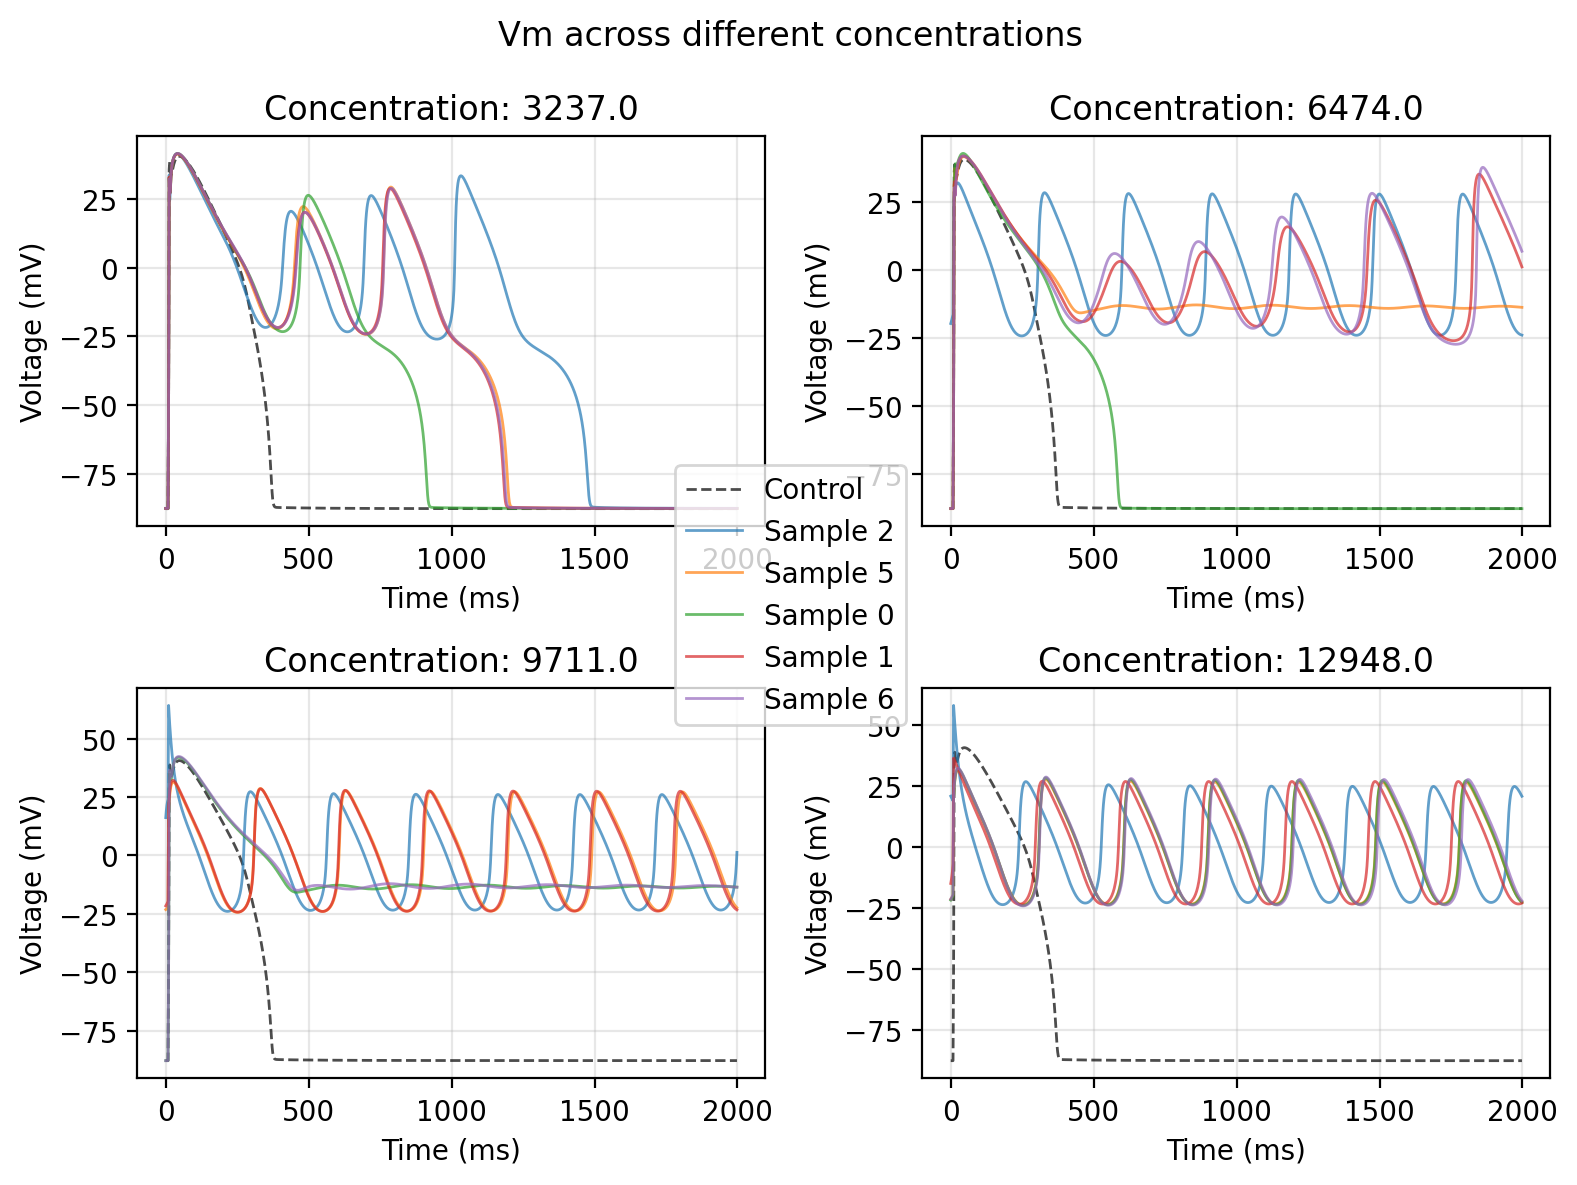
\includegraphics[scale=0.8]{./plots/time_series/quinidine/Vm_plot.png}
	\caption{Action potential result in various concentrations.}
	\label{fig:time_series_vm}
\end{figure}
\begin{figure}[H]
	\hspace{0.00cm}
	\centering
	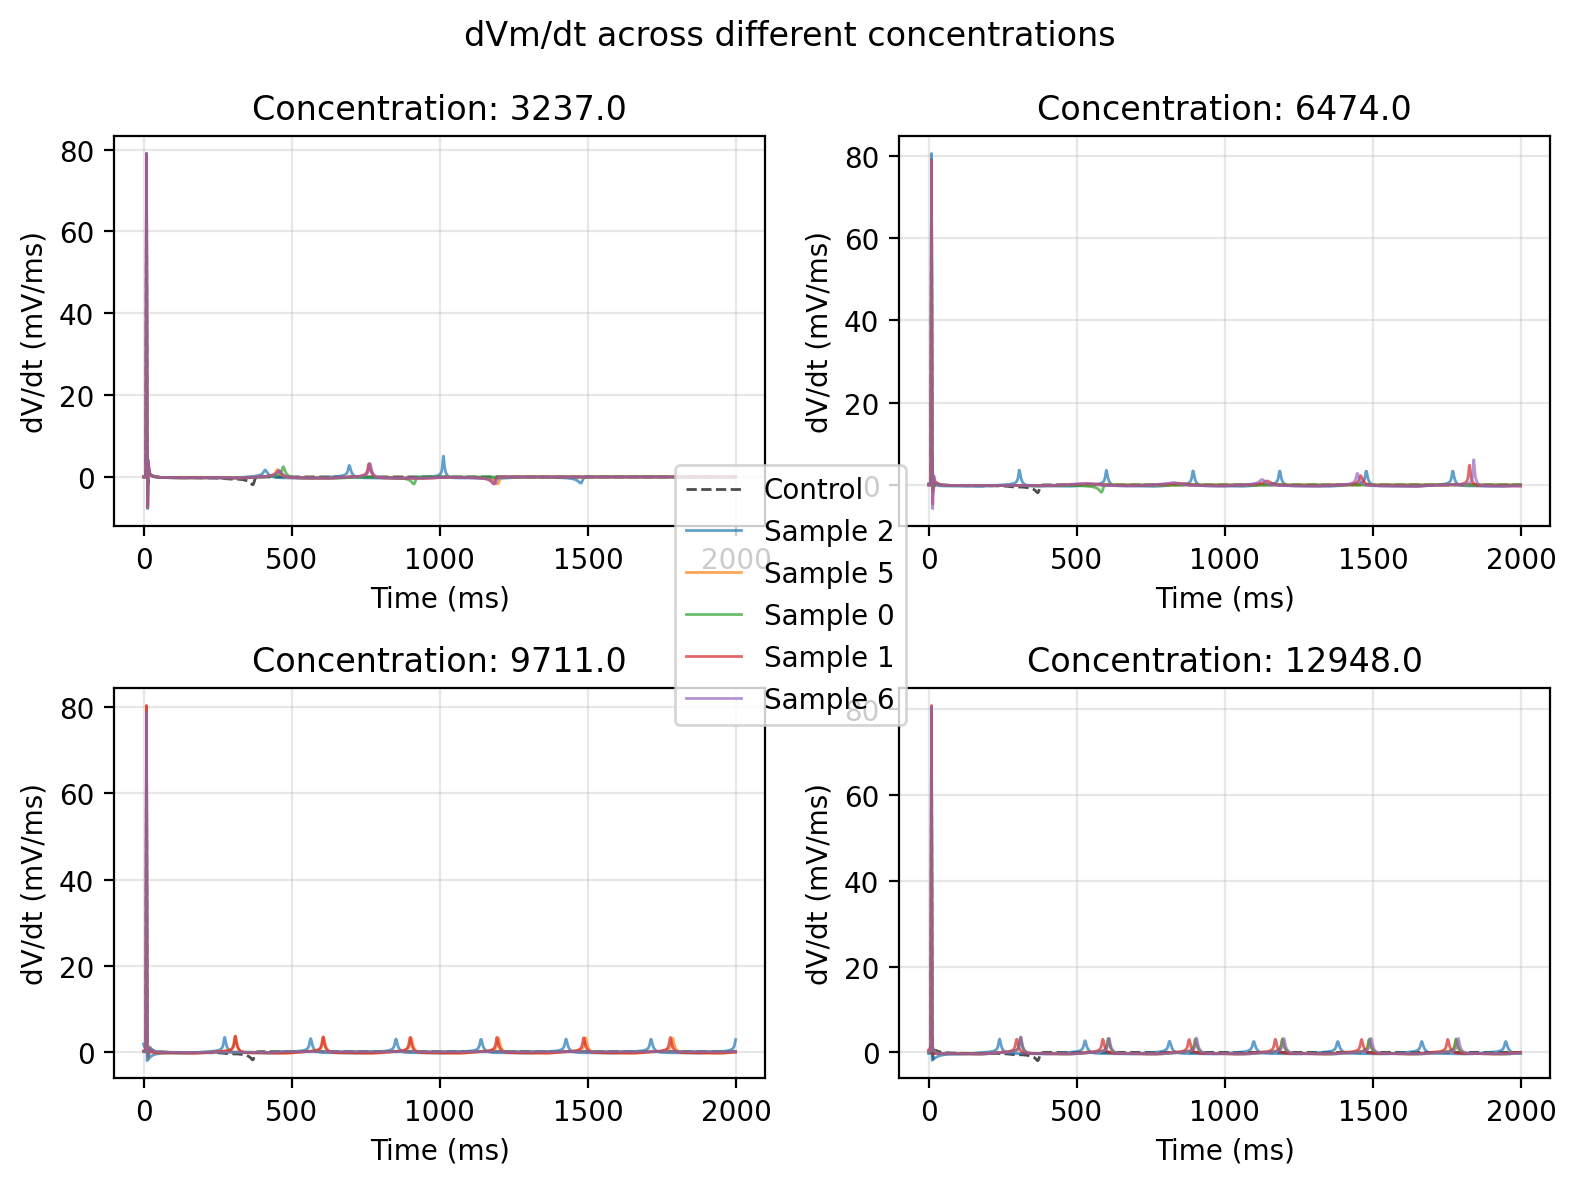
\includegraphics[scale=0.8]{./plots/time_series/quinidine/dVm_dt_plot.png}
	\caption{Rates of action potential result in various concentrations.}
	\label{fig:time_series_dvmdt}
\end{figure}
\begin{figure}[H]
	\hspace{0.00cm}
	\centering
	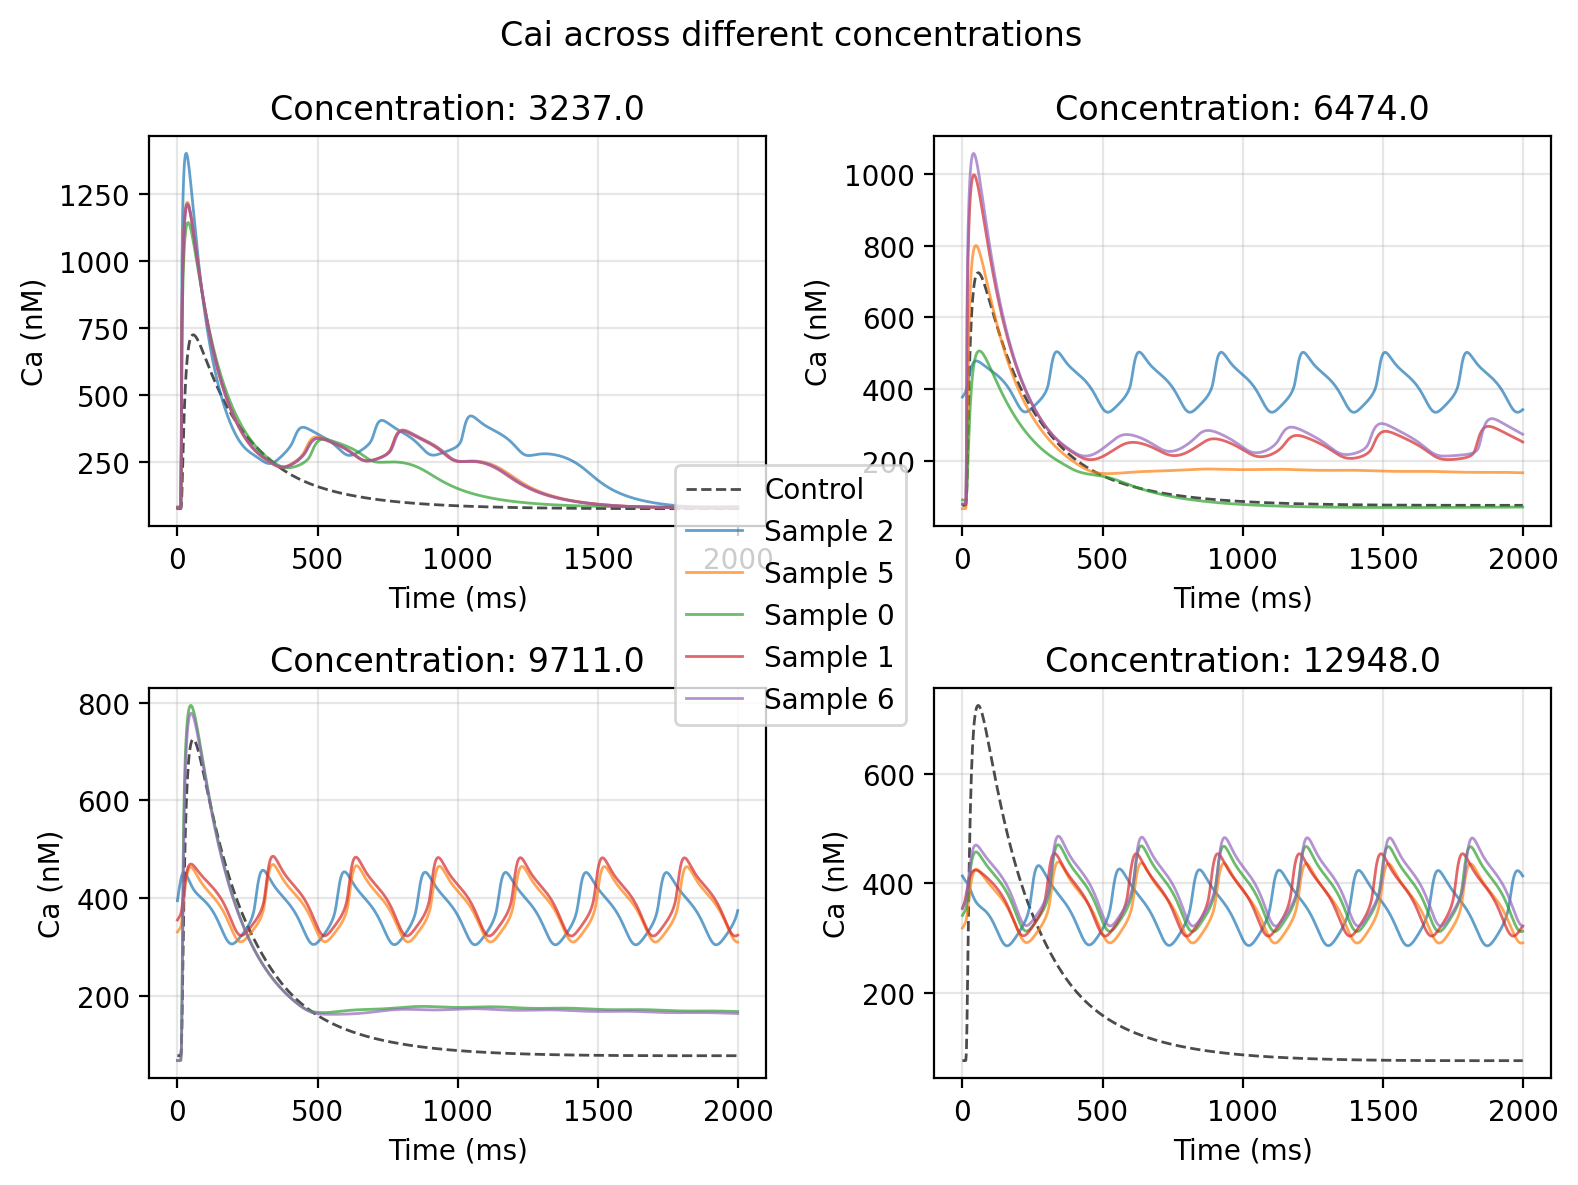
\includegraphics[scale=0.8]{./plots/time_series/quinidine/Cai_plot.png}
	\caption{Intracellular calcium concentration result in various concentrations.}
	\label{fig:time_series_cai}
\end{figure}
\begin{figure}[H]
	\hspace{0.00cm}
	\centering
	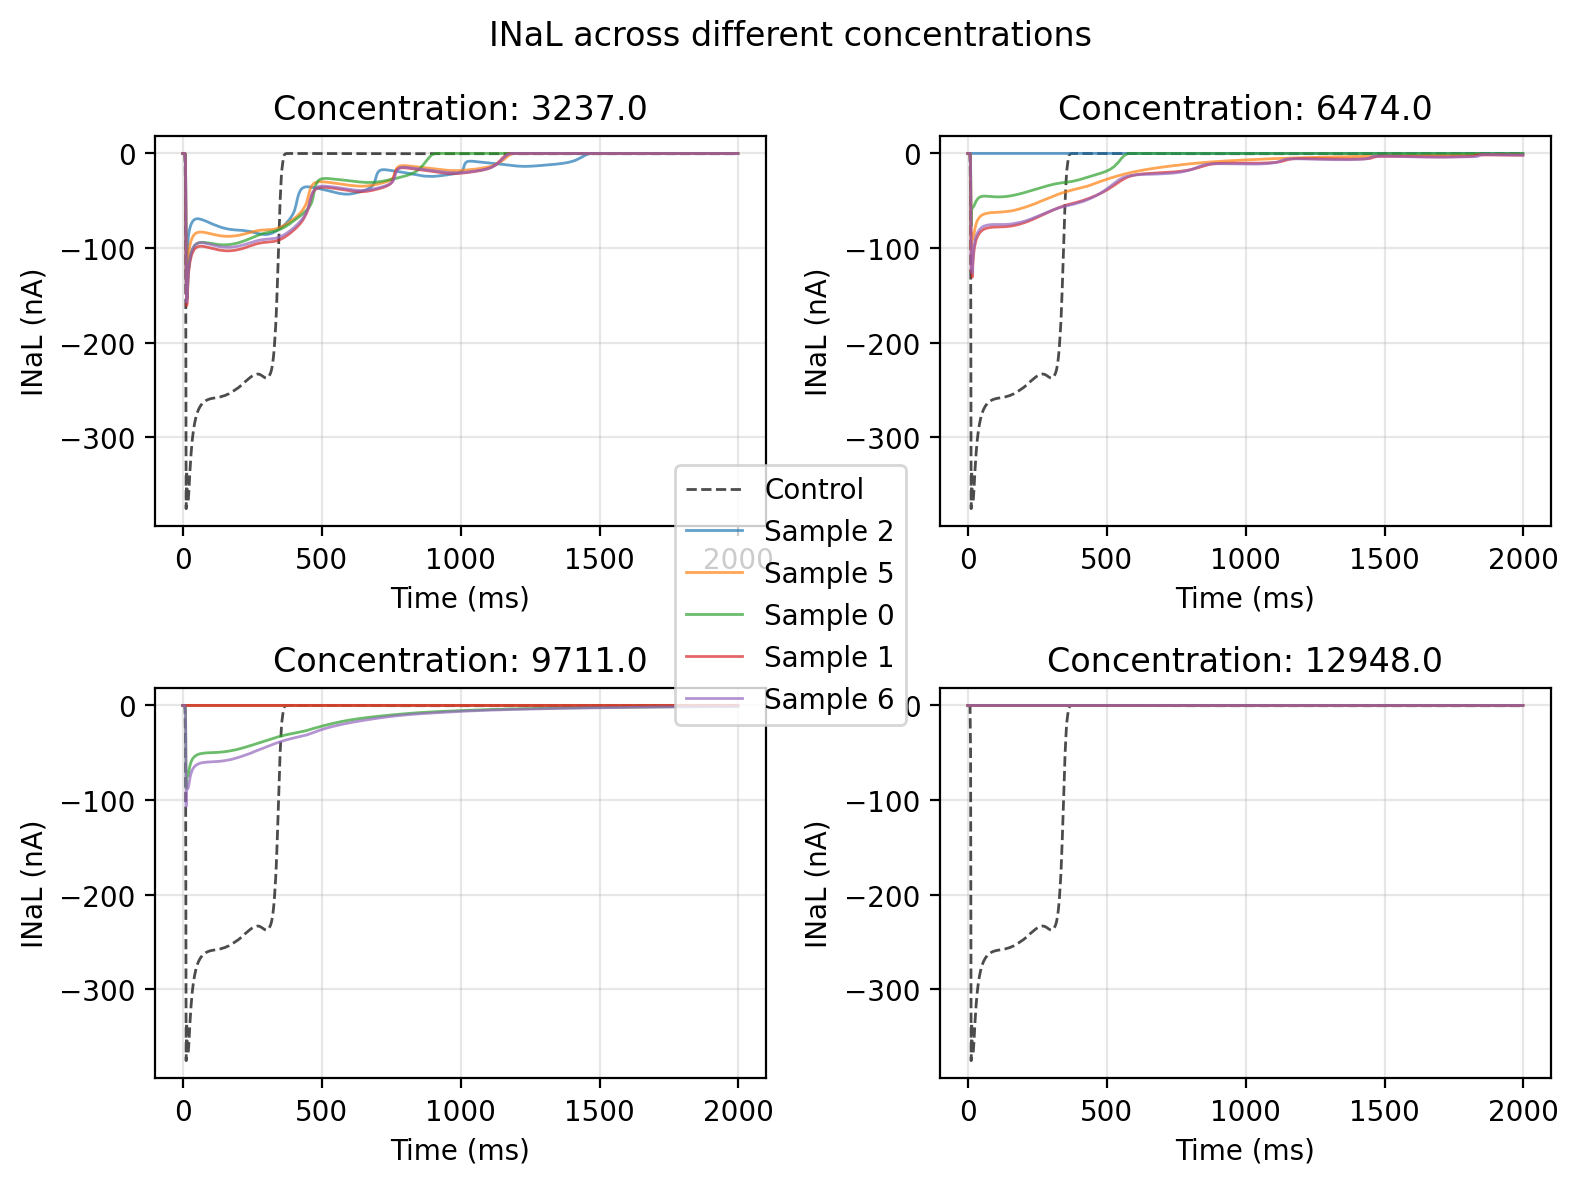
\includegraphics[scale=0.8]{./plots/time_series/quinidine/INaL_plot.png}
	\caption{L-type sodium current result in various concentrations.}
	\label{fig:time_series_inal}
\end{figure}
\begin{figure}[H]
	\hspace{0.00cm}
	\centering
	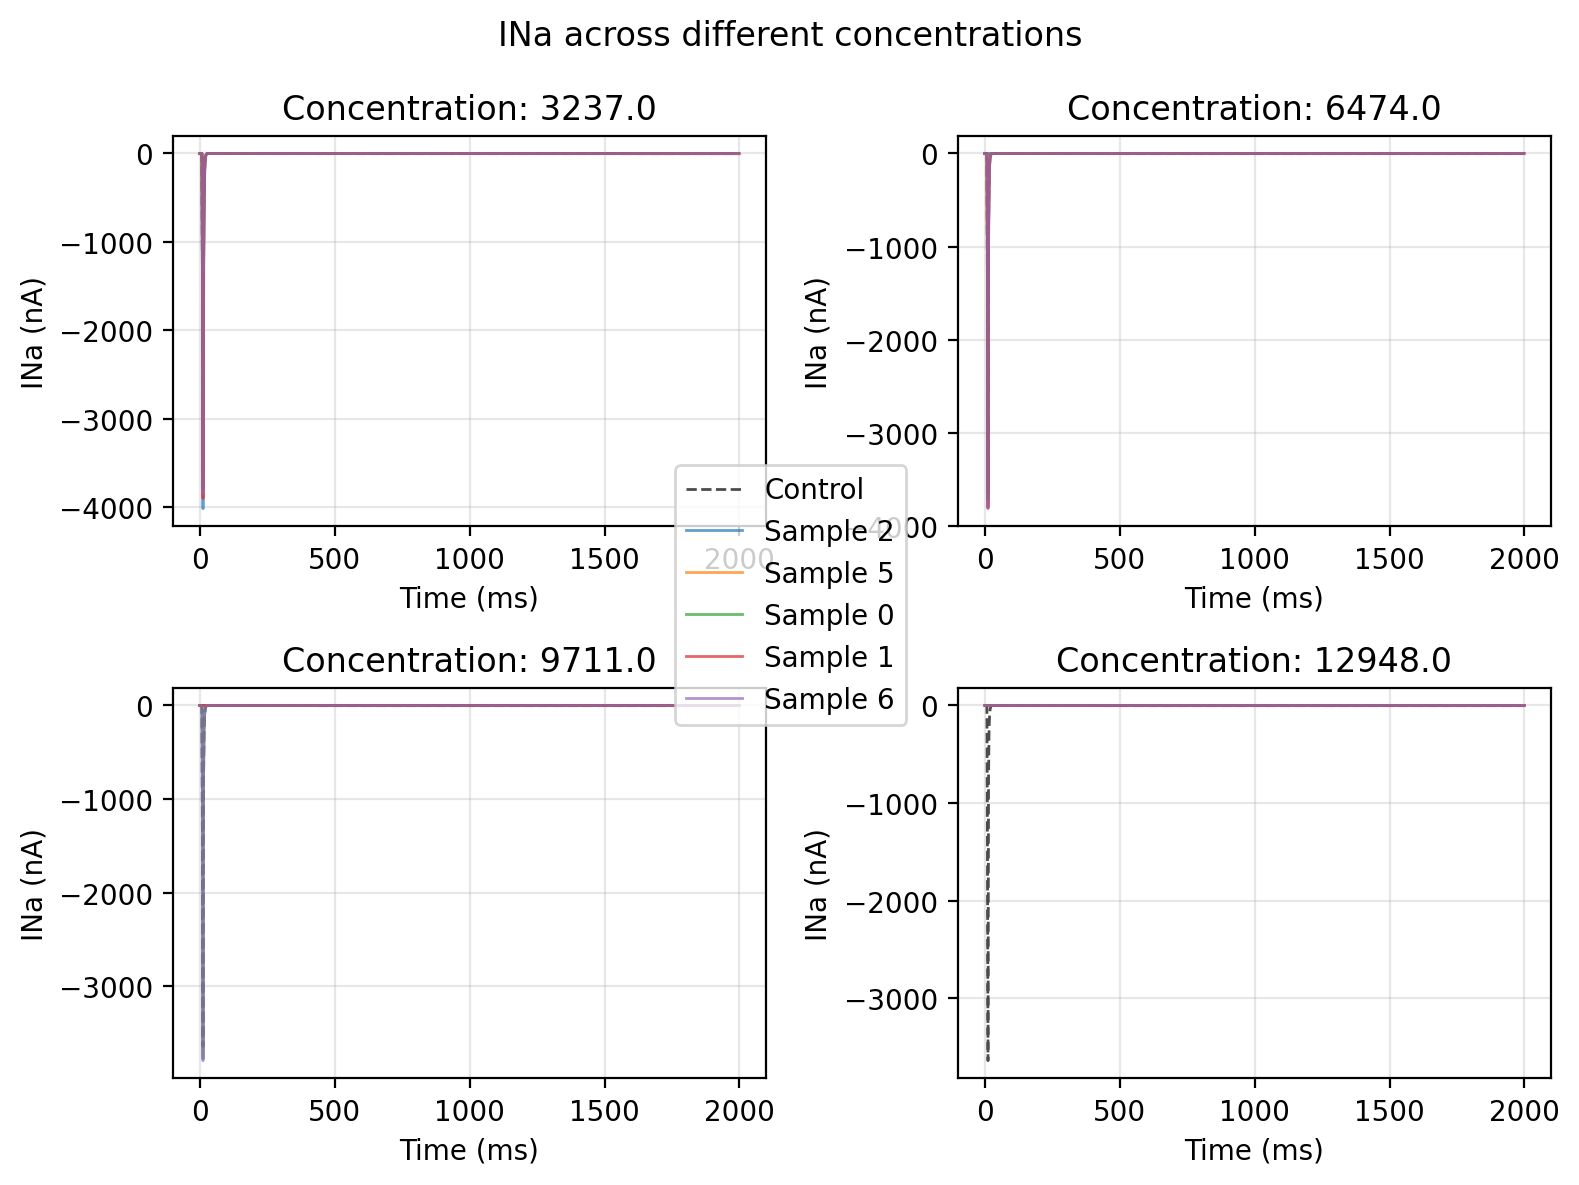
\includegraphics[scale=0.8]{./plots/time_series/quinidine/INa_plot.png}
	\caption{Sodium current result in various concentrations.}
	\label{fig:time_series_ina}
\end{figure}
\begin{figure}[H]
	\hspace{0.00cm}
	\centering
	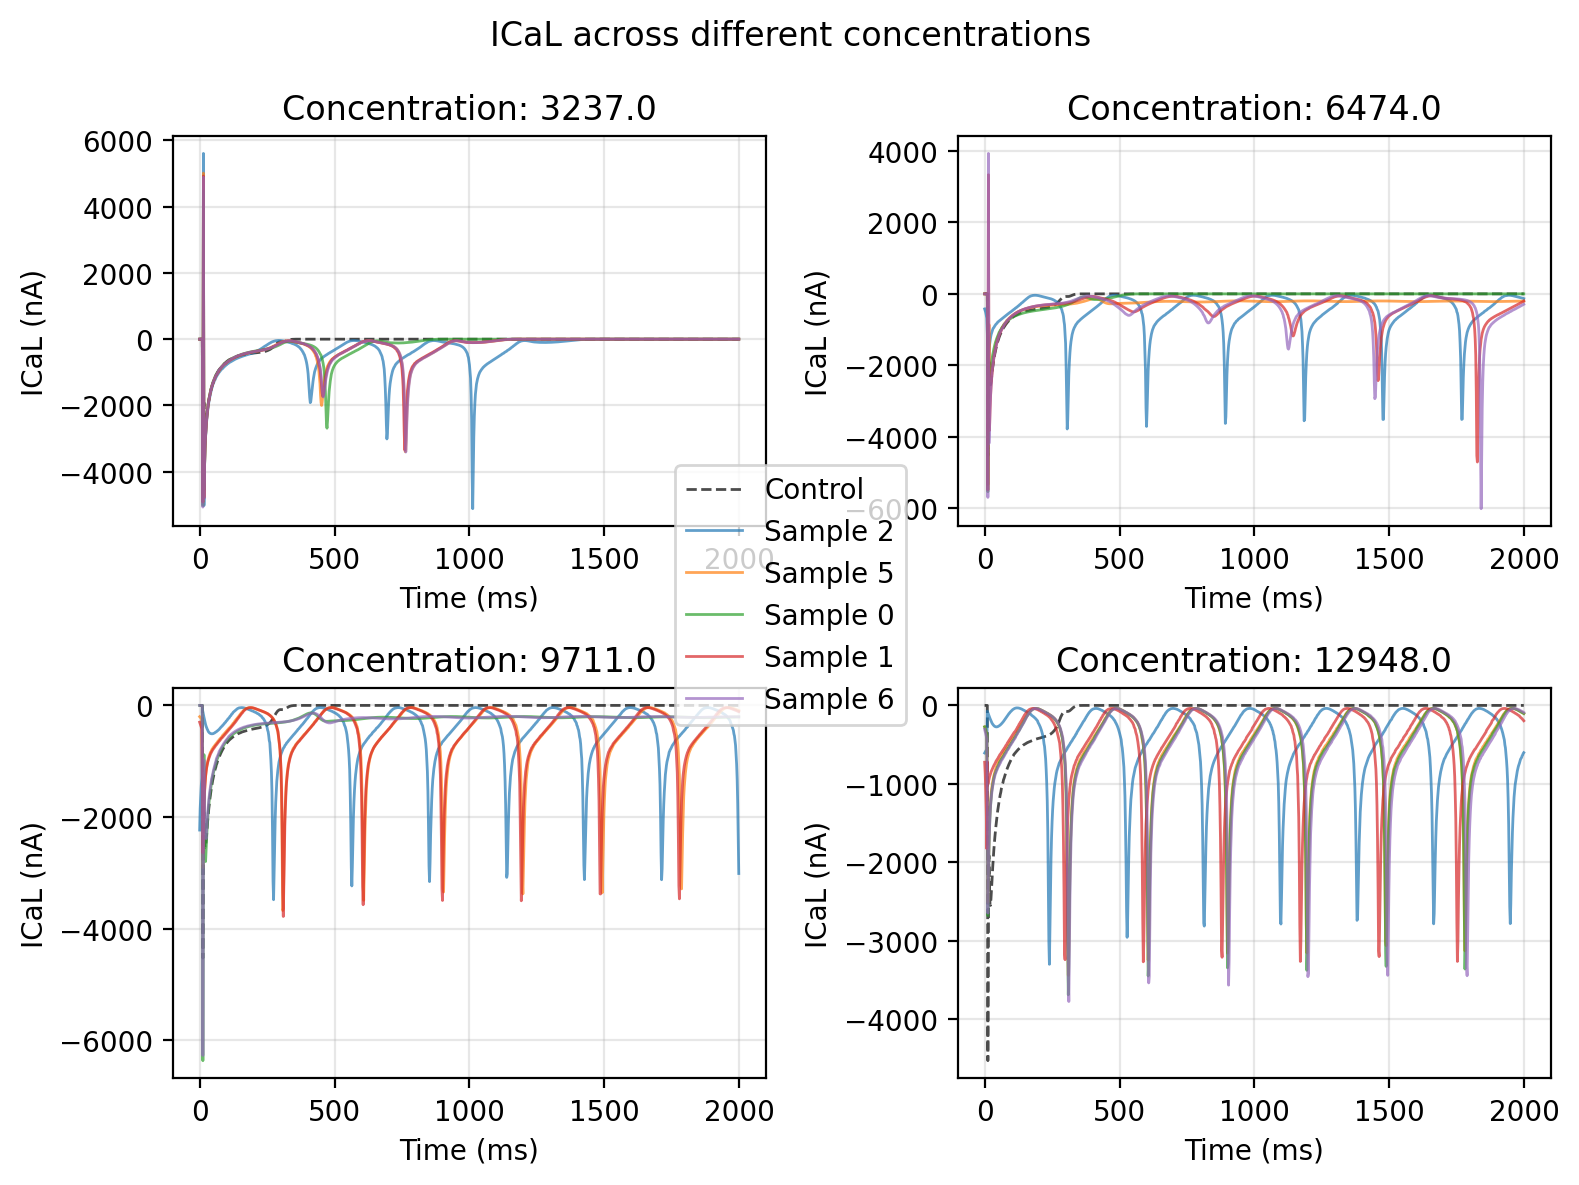
\includegraphics[scale=0.8]{./plots/time_series/quinidine/ICaL_plot.png}
	\caption{L-type calcium current result in various concentrations.}
	\label{fig:time_series_ical}
\end{figure}
\begin{figure}[H]
	\hspace{0.00cm}
	\centering
	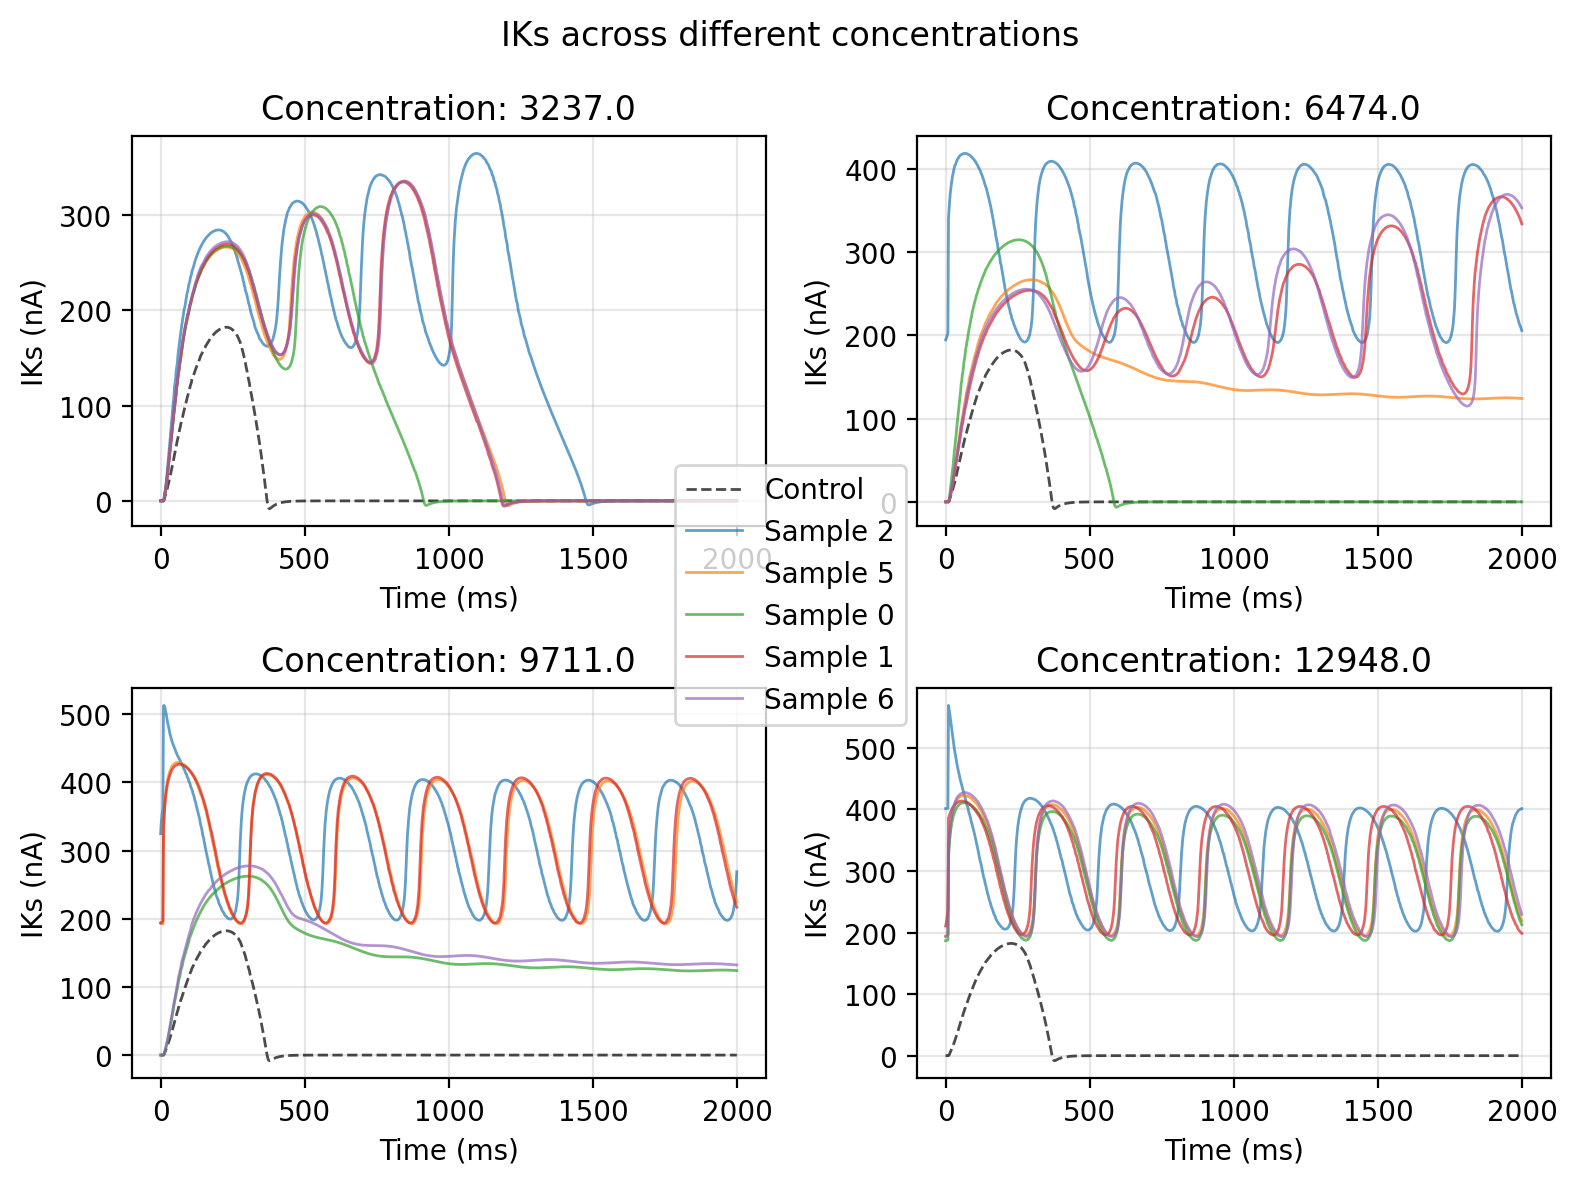
\includegraphics[scale=0.8]{./plots/time_series/quinidine/IKs_plot.png}
	\caption{Slow potassium current result in various concentrations.}
	\label{fig:time_series_iks}
\end{figure}
\begin{figure}[H]
	\hspace{0.00cm}
	\centering
	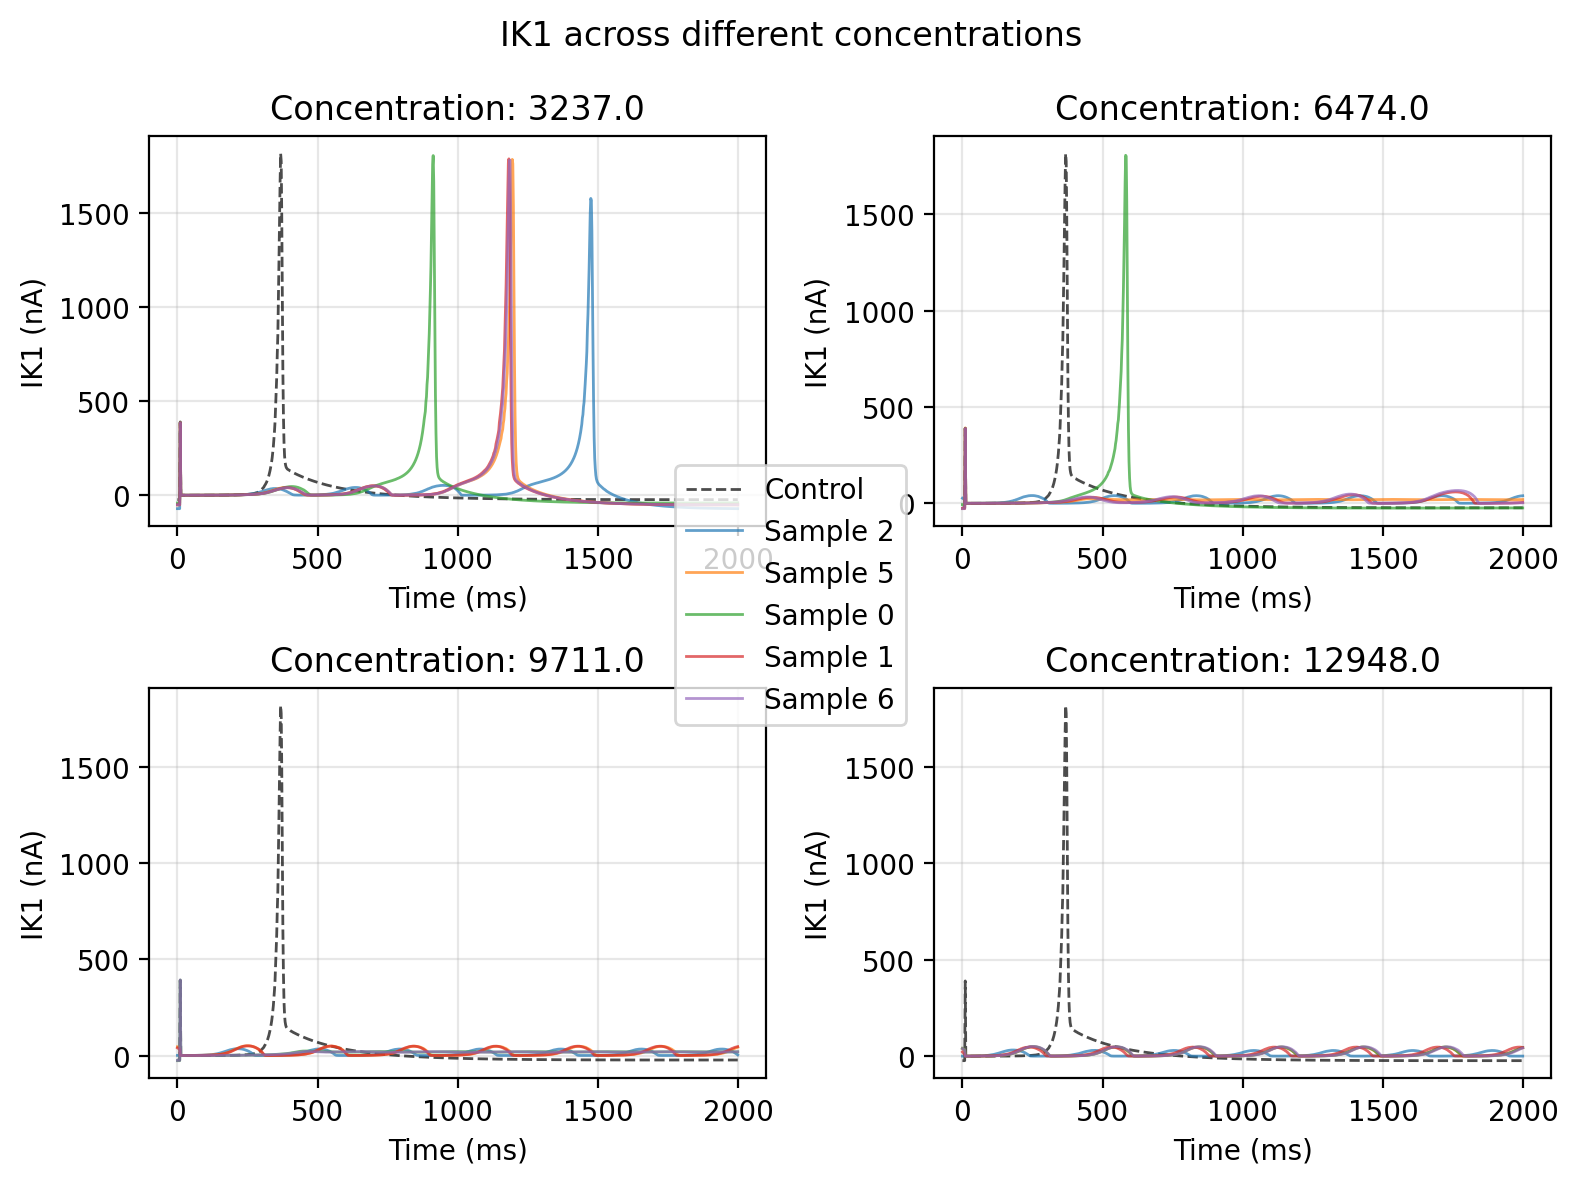
\includegraphics[scale=0.8]{./plots/time_series/quinidine/IK1_plot.png}
	\caption{Inward rectifier current result in various concentrations.}
	\label{fig:time_series_ik1}
\end{figure}
\begin{figure}[H]
	\hspace{0.00cm}
	\centering
	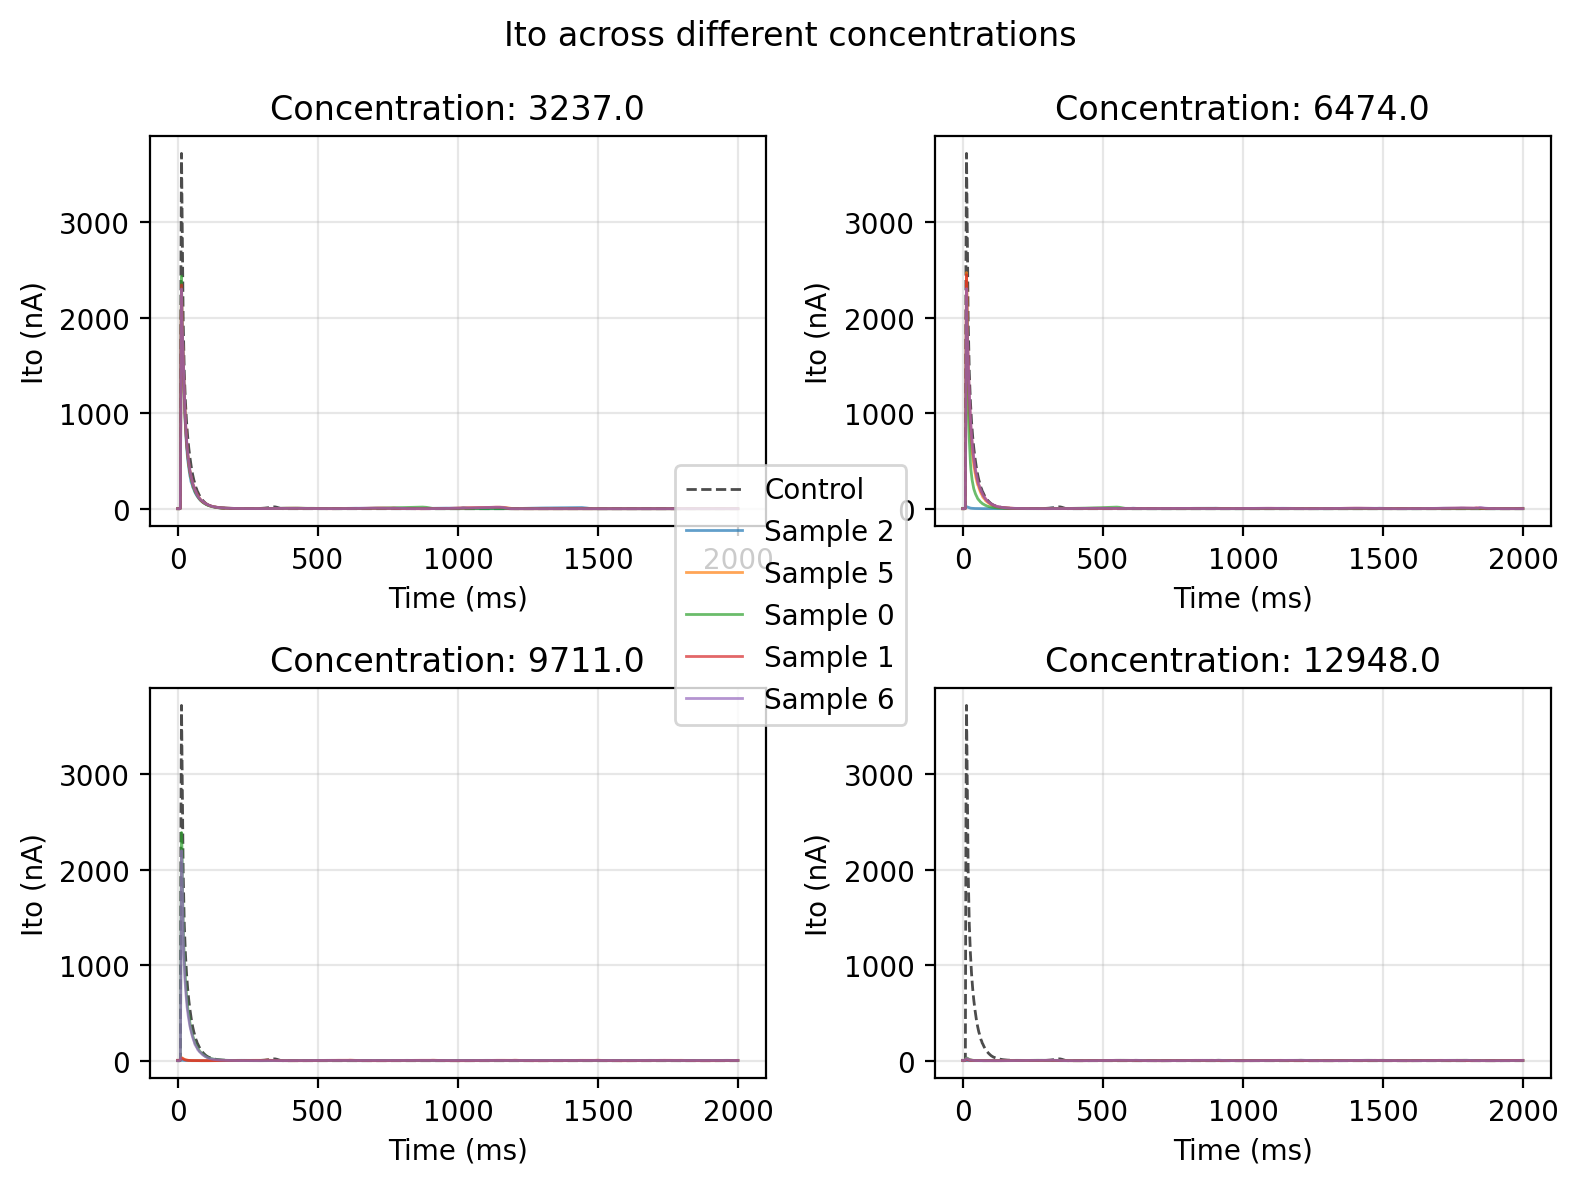
\includegraphics[scale=0.8]{./plots/time_series/quinidine/Ito_plot.png}
	\caption{Transient outward current result in various concentrations.}
	\label{fig:time_series_ito}
\end{figure}
\begin{figure}[H]
	\hspace{0.00cm}
	\centering
	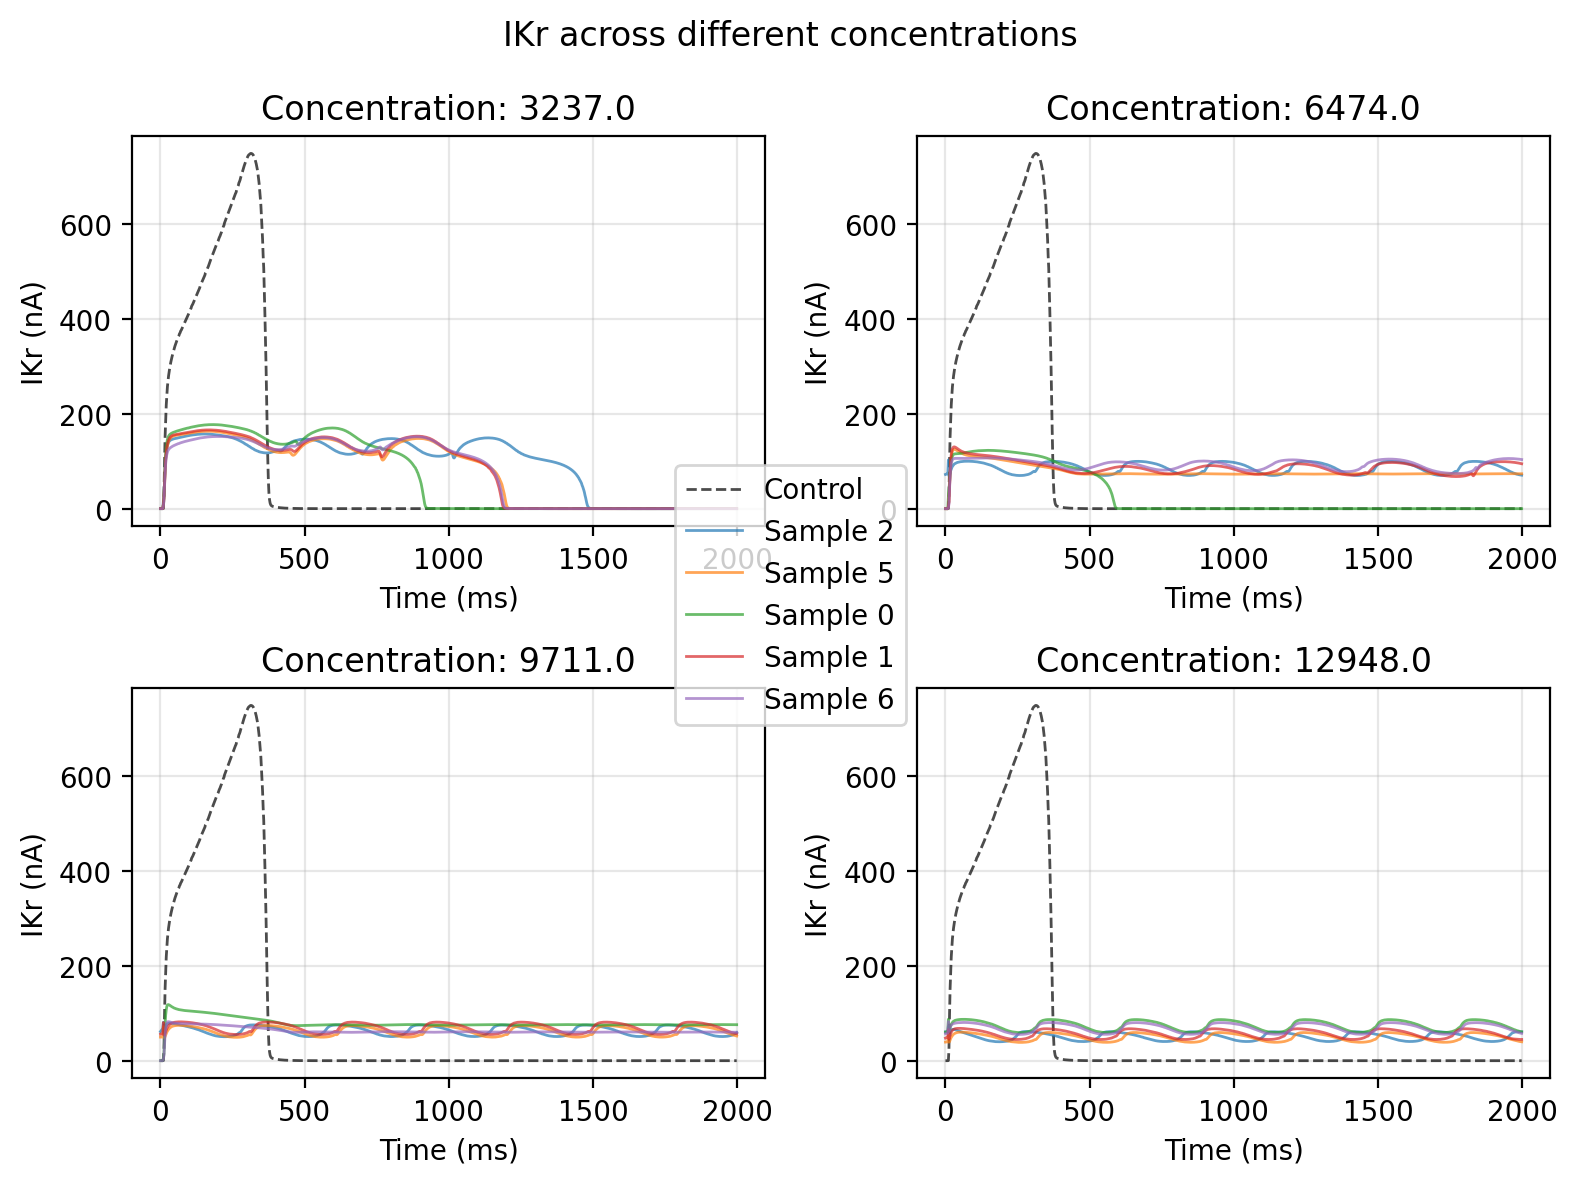
\includegraphics[scale=0.8]{./plots/time_series/quinidine/IKr_plot.png}
	\caption{hERG current result in various concentrations.}
	\label{fig:time_series_ikr}
\end{figure}
\begin{figure}[H]
	\hspace{0.00cm}
	\centering
	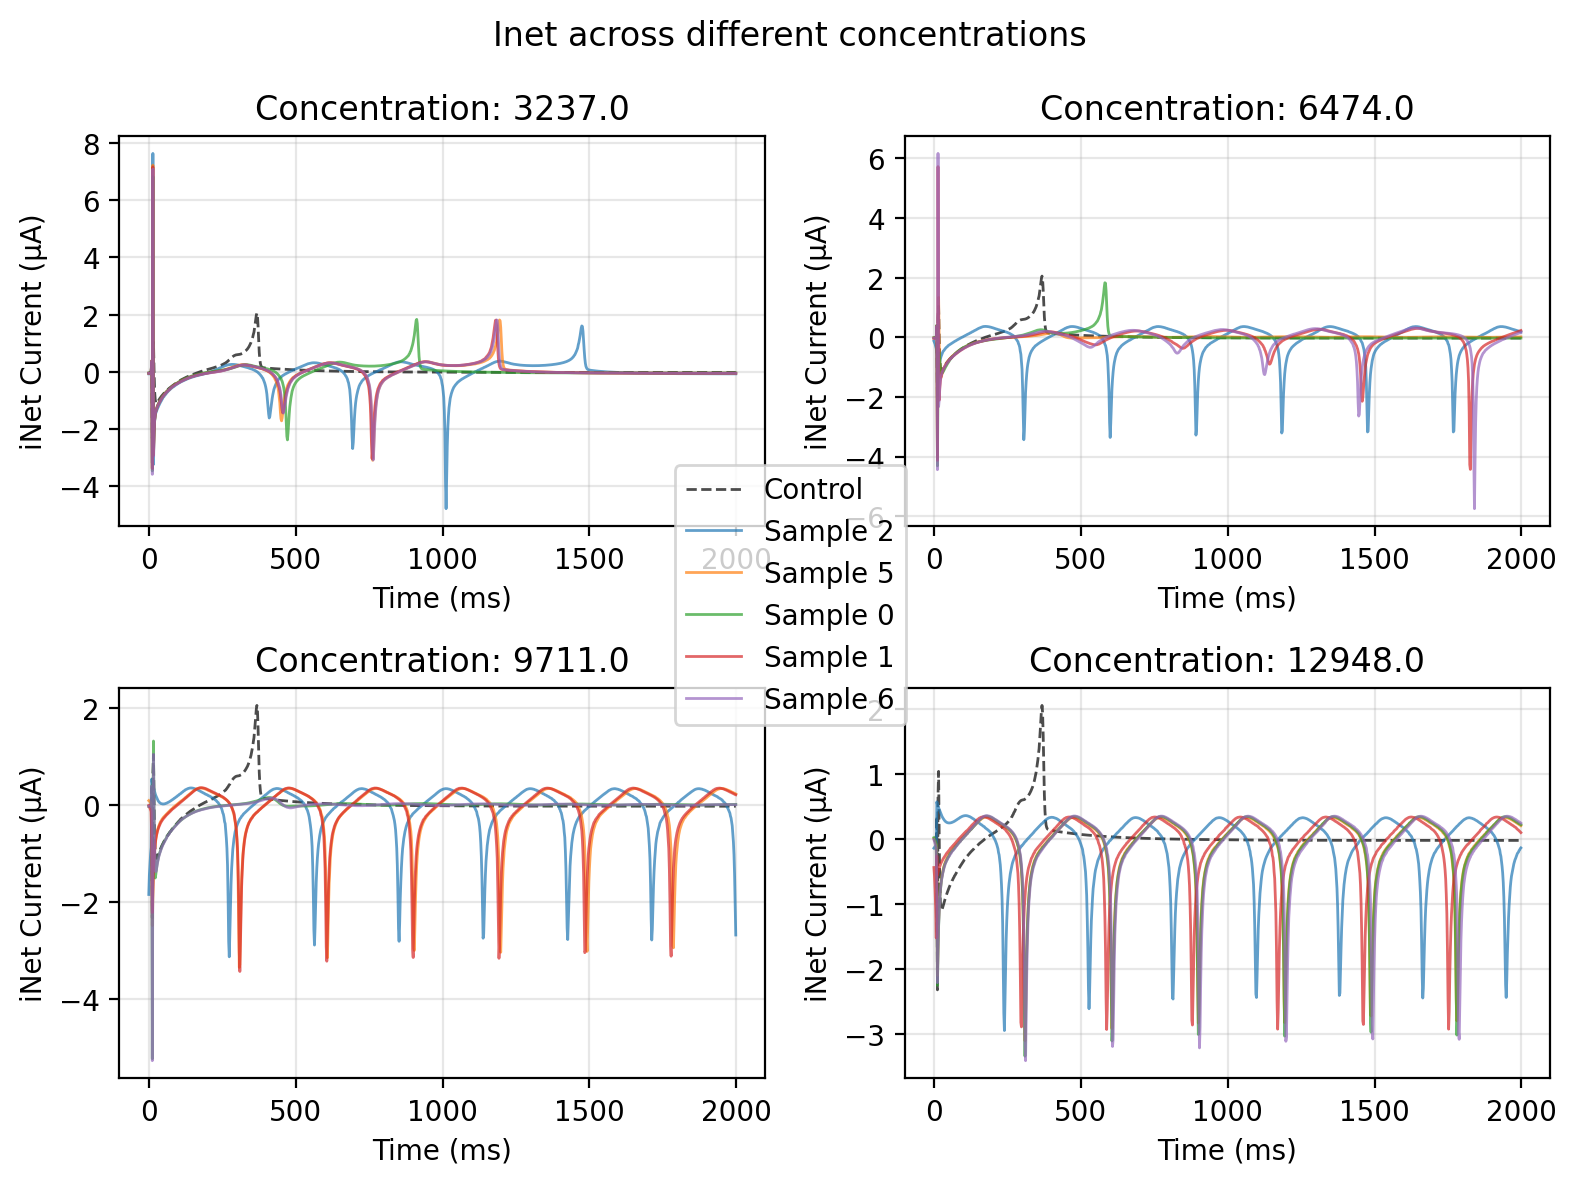
\includegraphics[scale=0.8]{./plots/time_series/quinidine/Inet_plot.png}
	\caption{Cummulative current result (iNet) in various concentrations.}
	\label{fig:time_series_inet}
\end{figure}
\subsection*{Feature Distribution}
The biomarker for cardiotoxicity assessment proposed by the US FDA Leading Study Group is qNet, and the following figures show the distribution of qNet and other features.
\begin{figure}[H]
	\hspace{0.00cm}
	\centering
	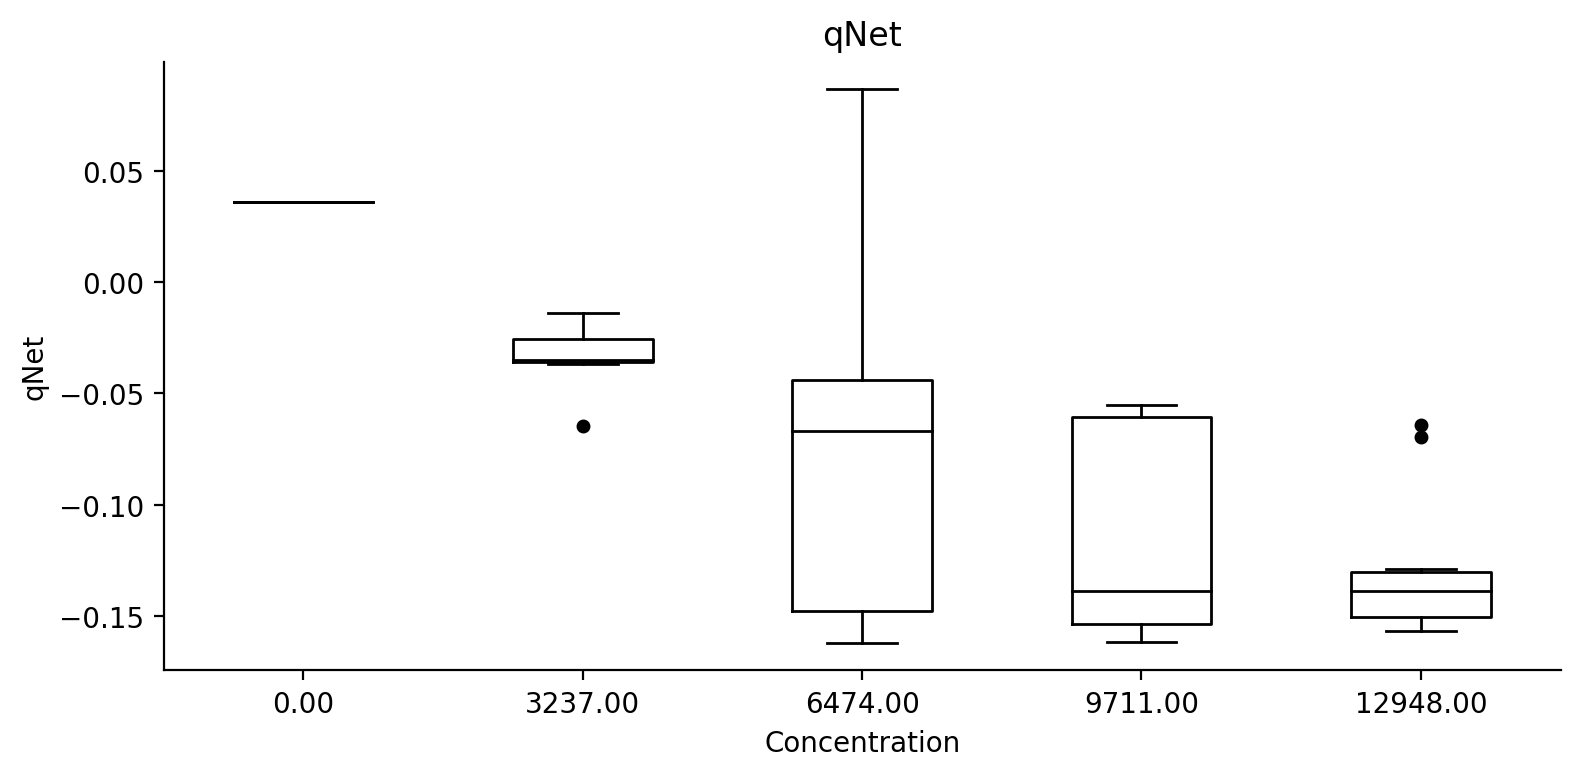
\includegraphics[scale=0.8]{./plots/features/quinidine/qnet_boxplot.png}
	\caption{qNet value distributions among several concentrations.}
	\label{fig:features_qnet}
\end{figure}
\begin{figure}[H]
	\hspace{0.00cm}
	\centering
	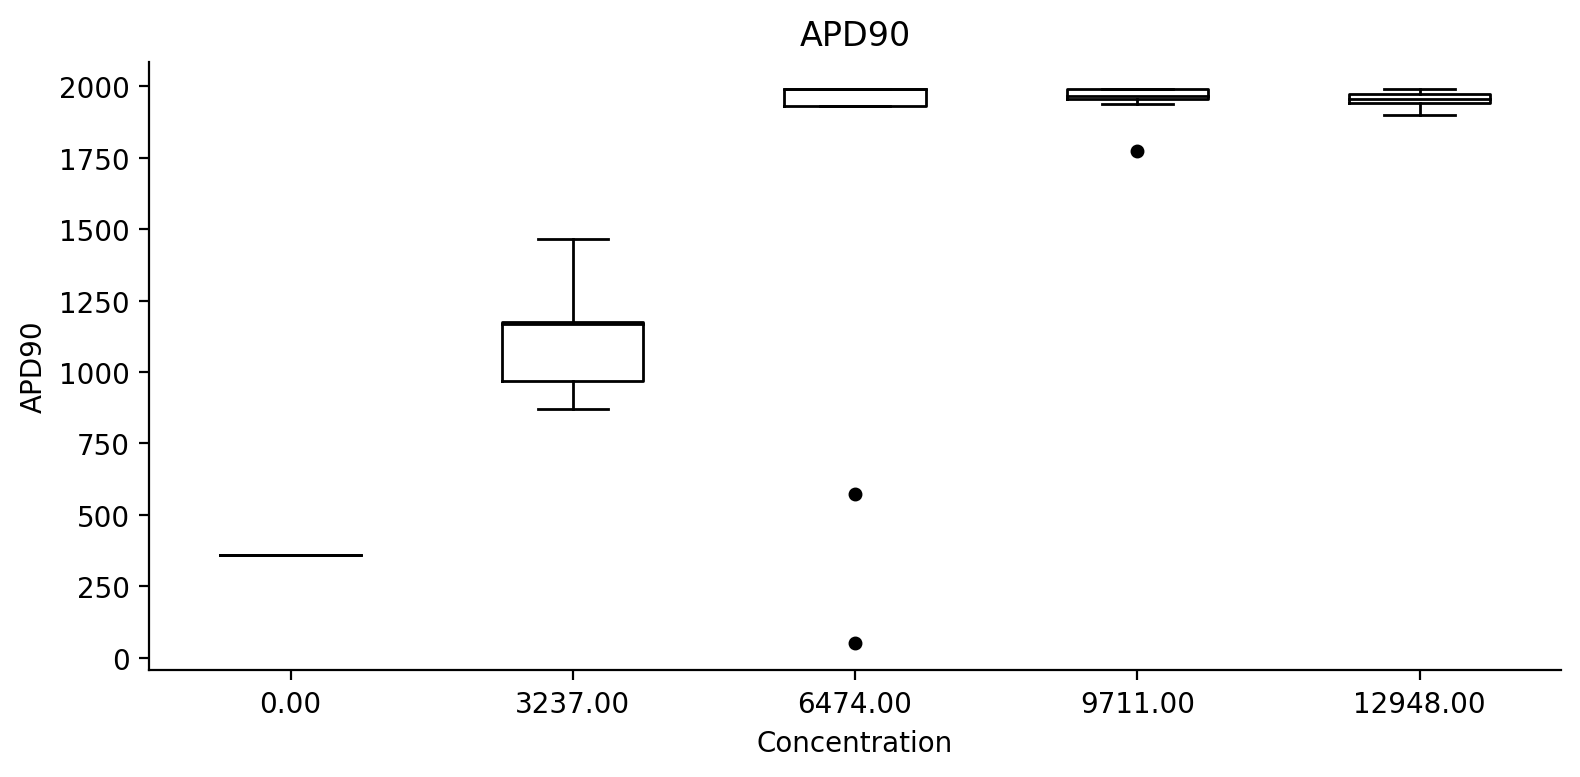
\includegraphics[scale=0.8]{./plots/features/quinidine/apd90_boxplot.png}
	\caption{APD90 value distributions among several concentrations.}
	\label{fig:features_apd90}
\end{figure}
\begin{figure}[H]
	\hspace{0.00cm}
	\centering
	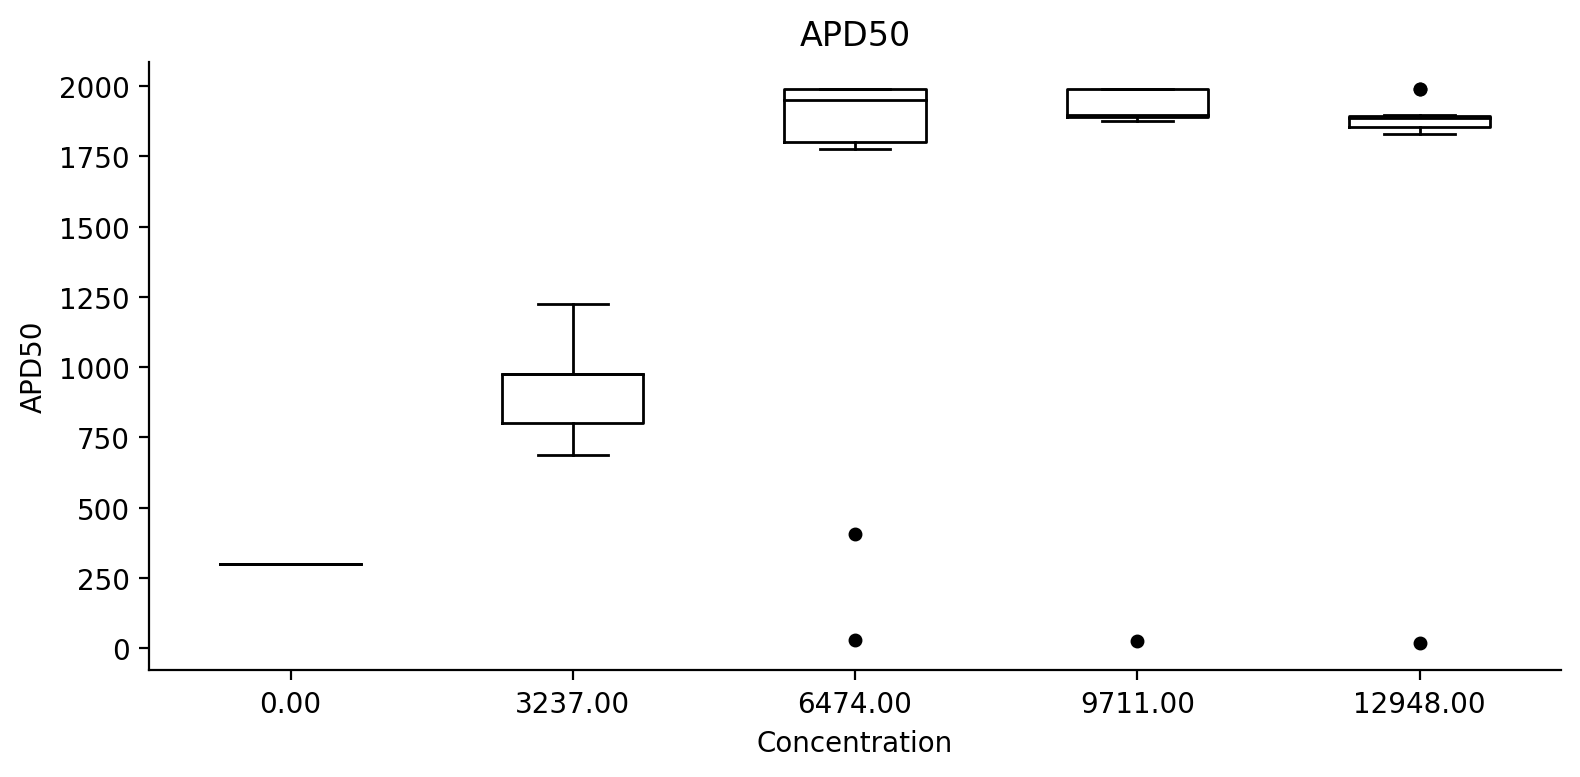
\includegraphics[scale=0.8]{./plots/features/quinidine/apd50_boxplot.png}
	\caption{APD50 value distributions among several concentrations.}
	\label{fig:features_apd50}
\end{figure}
\begin{figure}[H]
	\hspace{0.00cm}
	\centering
	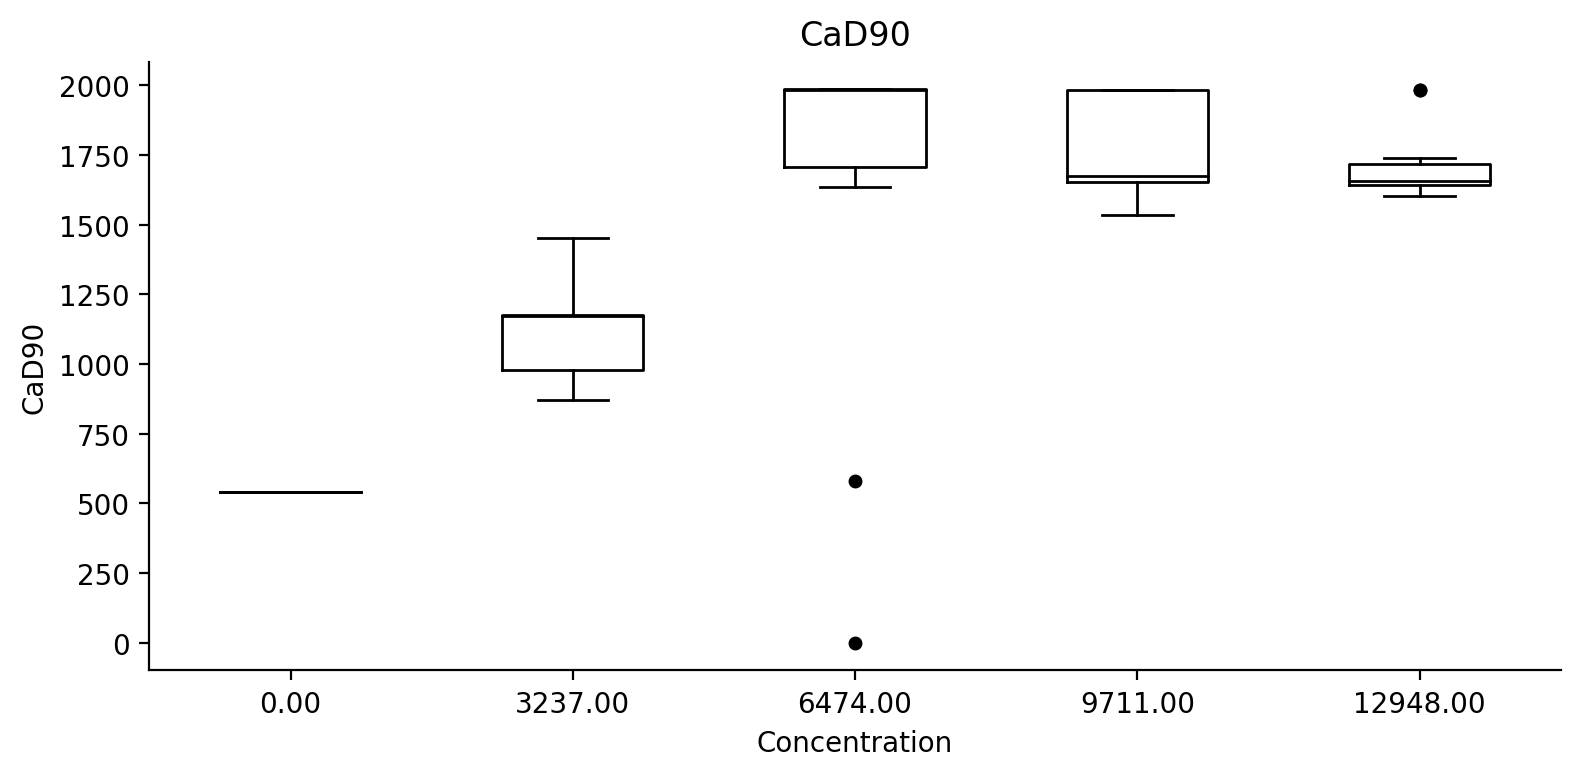
\includegraphics[scale=0.8]{./plots/features/quinidine/cad90_boxplot.png}
	\caption{CaD90 value distributions among several concentrations.}
	\label{fig:features_cad90}
\end{figure}
\begin{figure}[H]
	\hspace{0.00cm}
	\centering
	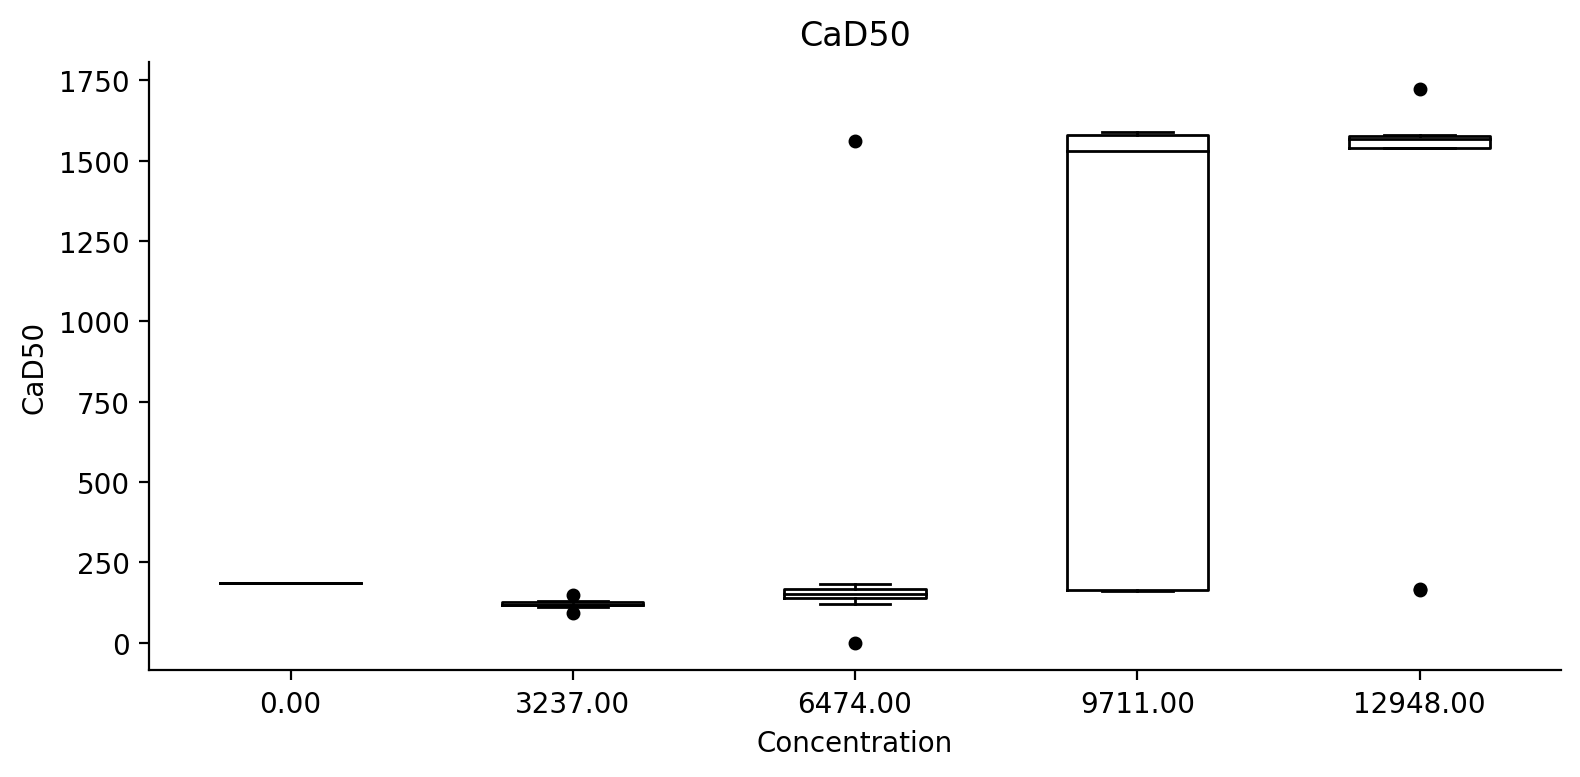
\includegraphics[scale=0.8]{./plots/features/quinidine/cad50_boxplot.png}
	\caption{CaD50 value distributions among several concentrations.}
	\label{fig:features_cad50}
\end{figure}
\begin{figure}[H]
	\hspace{0.00cm}
	\centering
	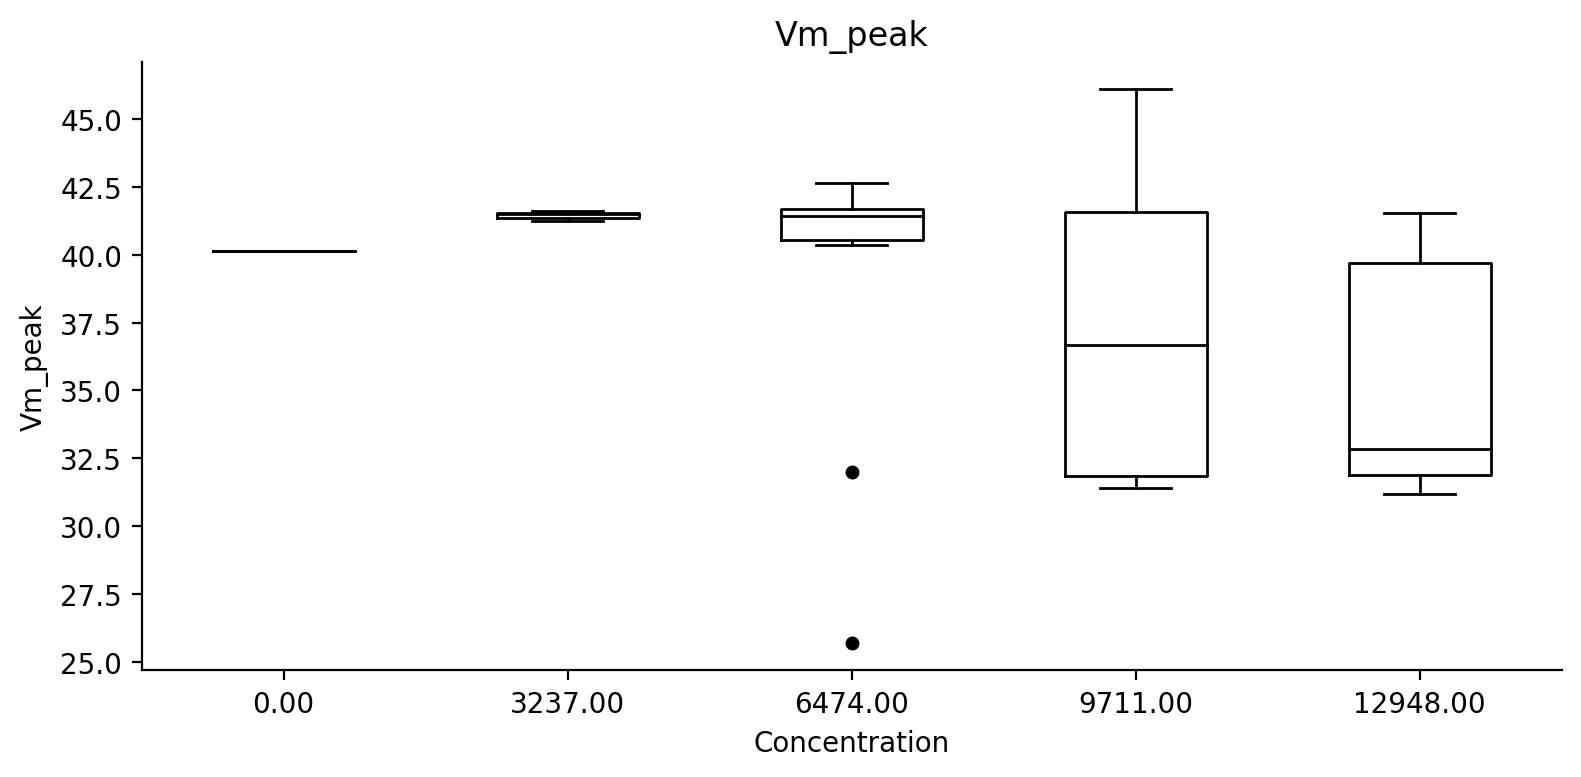
\includegraphics[scale=0.8]{./plots/features/quinidine/vm_peak_boxplot.png}
	\caption{Peak action potential value distributions among several concentrations.}
	\label{fig:features_vm_peak}
\end{figure}
\begin{figure}[H]
	\hspace{0.00cm}
	\centering
	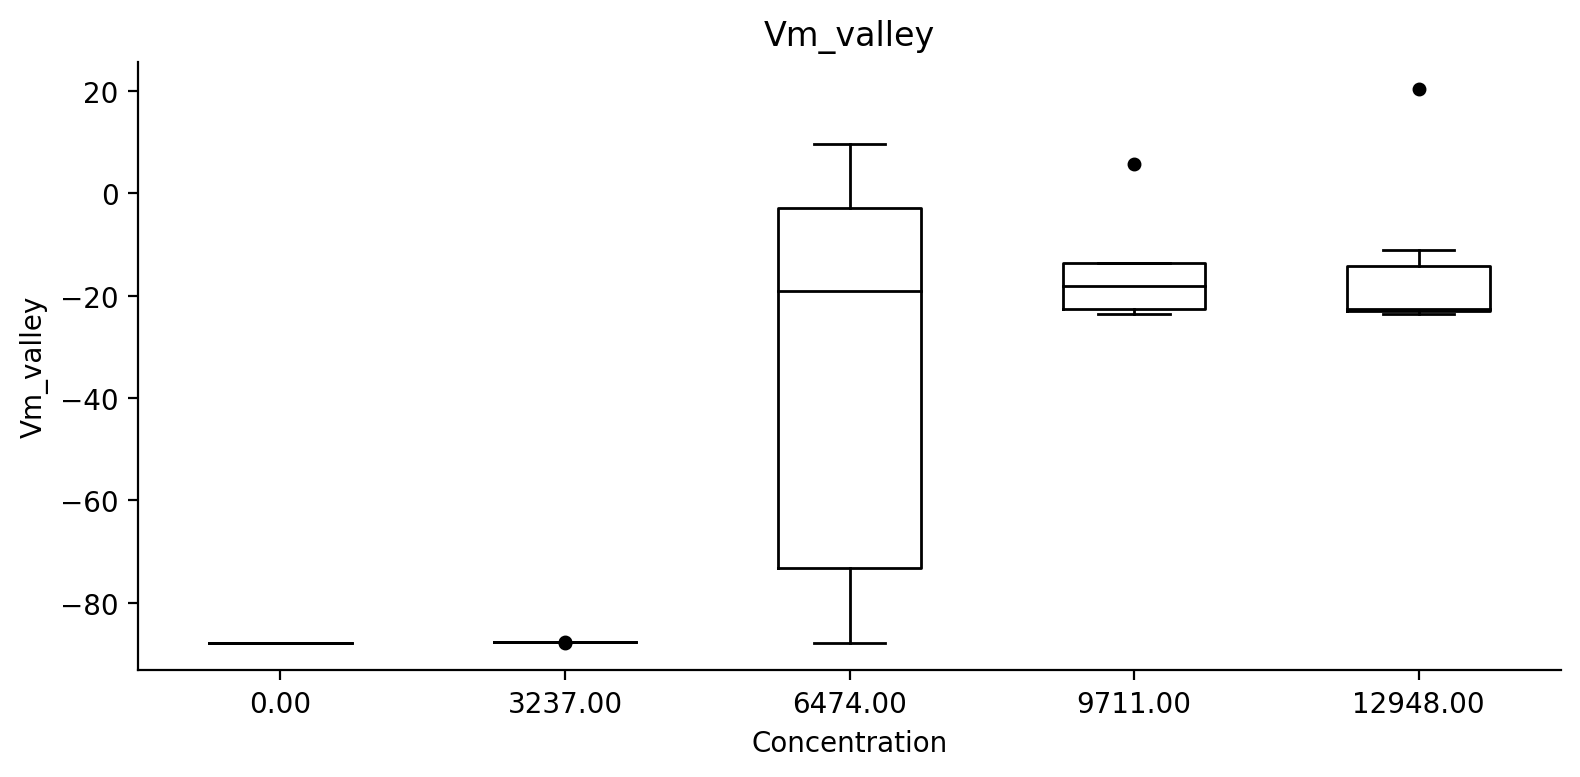
\includegraphics[scale=0.8]{./plots/features/quinidine/vm_valley_boxplot.png}
	\caption{Lowest action potential value distributions among several concentrations.}
	\label{fig:features_vm_valley}
\end{figure}
\begin{figure}[H]
	\hspace{0.00cm}
	\centering
	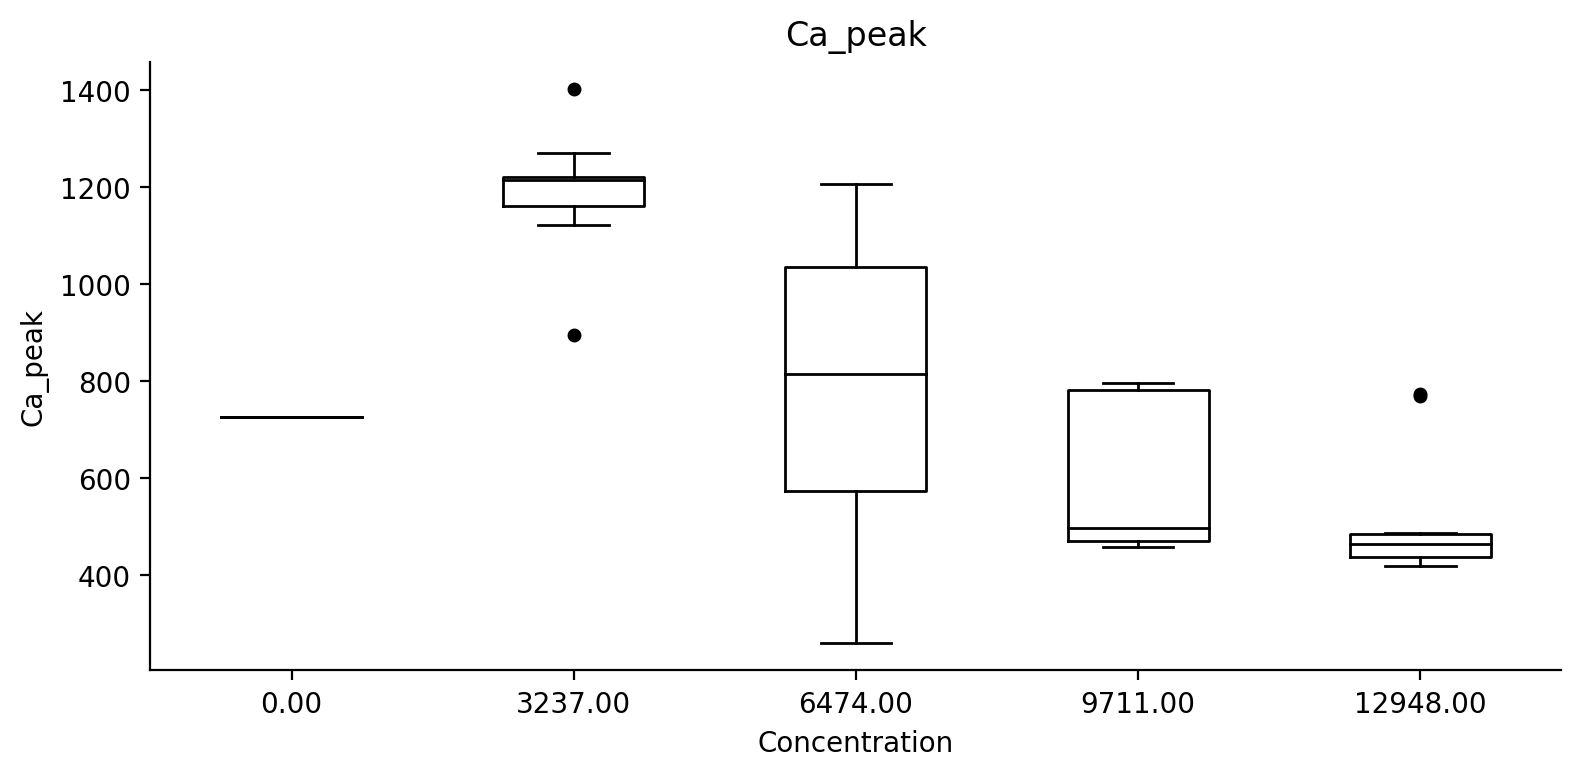
\includegraphics[scale=0.8]{./plots/features/quinidine/ca_peak_boxplot.png}
	\caption{Peak calcium concentration value distributions among several concentrations.}
	\label{fig:features_ca_peak}
\end{figure}
\begin{figure}[H]
	\hspace{0.00cm}
	\centering
	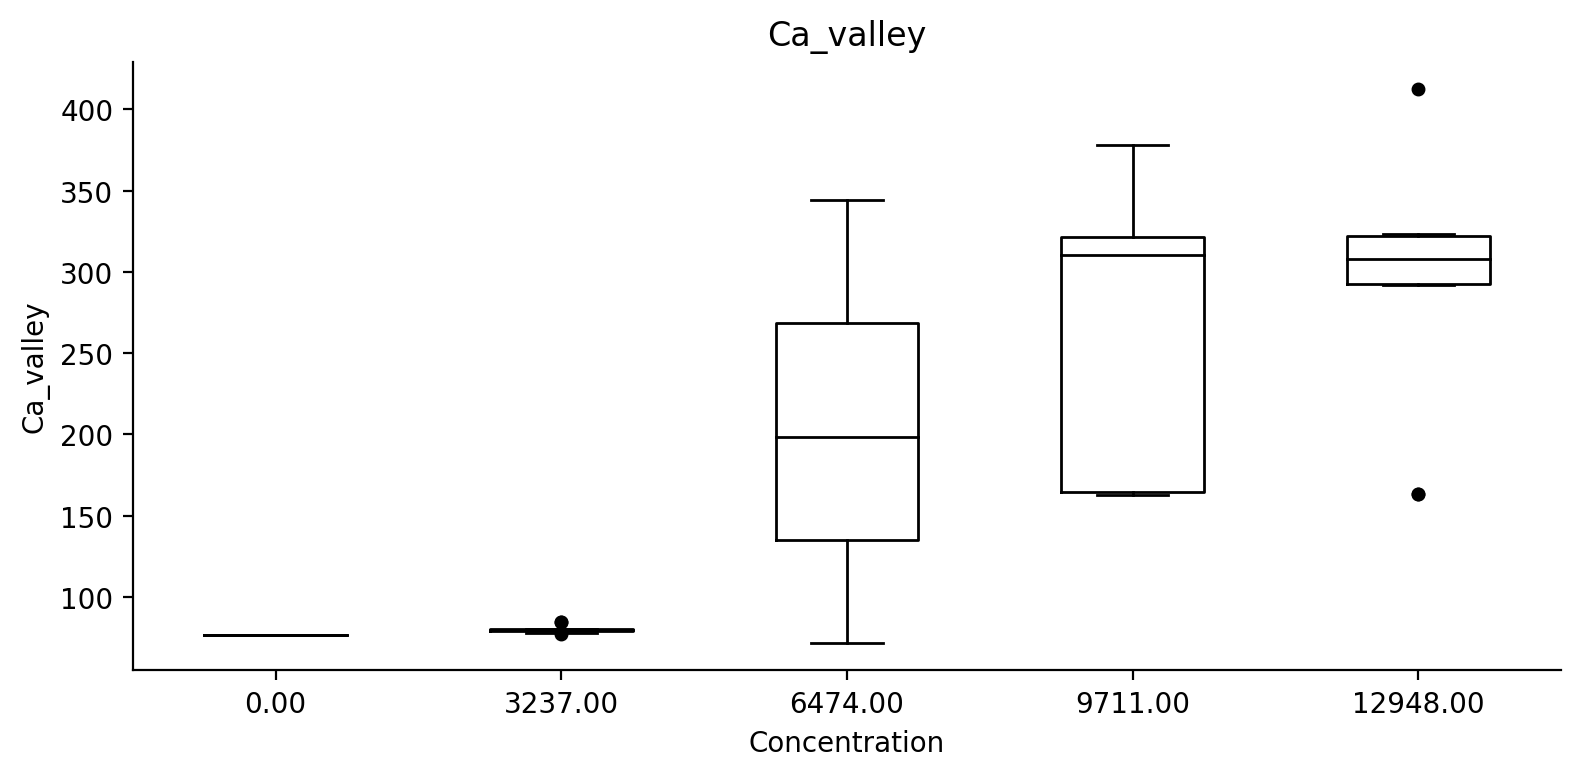
\includegraphics[scale=0.8]{./plots/features/quinidine/ca_valley_boxplot.png}
	\caption{Lowest calcium concentration value distributions among several concentrations.}
	\label{fig:features_ca_valley}
\end{figure}

\end{document}
